\documentclass[18pt]{beamer}
\usepackage[utf8]{inputenc}
\usepackage{xcolor}
\usepackage{hyperref}
\usepackage{templates/mytemplate}
\usepackage{templates/beamerthemekit}
\usepackage{graphicx}
\usepackage{microtype}
\usepackage{listings}
\usepackage{multicol}
\usepackage{siunitx}
\usepackage{physics}
\usepackage{appendixnumberbeamer}
\usepackage{booktabs}
\usepackage{longtable}
\usepackage{amssymb}
\usepackage{todonotes}

\lstset{ %
  backgroundcolor=\color{white},   % choose the background color; you must add \usepackage{color} or \usepackage{xcolor}; should come as last argument
  basicstyle=\tiny\ttfamily,
  xleftmargin=-10pt,
  breaklines=false,                 % sets automatic line breaking
  captionpos=b,                    % sets the caption-position to bottom
  % frame=single,	                   % adds a frame around the code
  keepspaces=true,                 % keeps spaces in text, useful for keeping indentation of code (possibly needs columns=flexible)
  language=C++,                 % the language of the code
  % morekeywords={*,...},            % if you want to add more keywords to the set
  tabsize=2,	                   % sets default tabsize to 2 spaces
  keywordstyle=\bfseries\color{kit-green70},
  commentstyle=\itshape\color{kit-blue70},
  identifierstyle=\color{black},
  stringstyle=\color{kit-orange100},  
}

\hypersetup{colorlinks=true, urlcolor=kit-blue100, %linkcolor=Firebrick4
}

\title{Einsichten in die Spurfindung an Belle II mit kosmischer Strahlung} 
\subtitle{Wissenschaftliches Schreiben und Präsentieren für Physiker und Metereologen}
\author{\underline{Michael Eliachevitch}}
\date{24. Januar 2018}
\titleimage{transparent}
\institute{}


\begin{document}
\selectlanguage{ngerman}

\begin{frame}
  \titlepage
\end{frame}

\begin{frame}
  \frametitle{Was ist Belle II}
  \begin{itemize}
    \item im Bau befindlicher Teilchendektor an dem SuperKEKB-Beschleuniger in Japan
    \item geplanter Beginn der Kollisionen: Frühjahr 2018
    \item physikalisches Ziel: Suche nach \emph{Physik jenseits des Standardmodells}
    \item experimentelles Ziel: Beobachtung der Zerfallskette aus dem Zerfall B-Mesonen mit hoher Präzision
    \item Abweichungen von theoretischen Vorhersagen $\rightarrow$ \emph{neue Physik}?
    \item \emph{Spurfindung}: Rekonstruktion der Teilchenbahnen der Zerfallsprodukte aus Rohdaten des Detektors
    \end{itemize}

    
    
\end{frame}

\begin{frame}
  \frametitle{Besonderheiten der Spurfindung an Belle II}
  \begin{itemize}
  \item SuperKEKB: Elektron-Positrion-Collider als \emph{B-Fabrik}:
    \begin{itemize}
    \item wenig Untergrund, typischerweise 7-11 Spuren 
    \item Kenntniss des Anfangszustandes: Erzeugt immer zwei B-Mesonen mit bekanntem Impuls
    \end{itemize}
    \begin{itemize}
    \item Herausforderungen:
      \begin{itemize}
      \item Ziel: \emph{alle} Spuren in einem Ereignis finden $\rightarrow$ sehr hohe Effizienz
      \item Kollisionsereignis etwa alle 4\,ns $\rightarrow$ hohe Performanz der Algorithmen
      \item Teilchen mit niedrigem Impuls
      \end{itemize}
    \end{itemize}
  \end{itemize}
  
\end{frame}

\begin{frame}
  \frametitle{Kosmische Strahlen an Belle II}
  
\end{frame}

\begin{frame}
  \frametitle{Prinzip: Datenbasierte Schätzung der Spurfindungs-Effizienz}
  \begin{itemize}
  \item typical cosmics event: single muon track, no secondaries
  \item cosmics passing through VXD volume create two \texttt{NonMergedRecoTracks}\\
    $\rightarrow$ in the following use those instead of merged \texttt{RecoTracks}
  \item idea: estimate finding efficiency from \textcolor{kit-red100}{finding fails} in events where \textcolor{kit-blue100}{two (findable) tracks are expected}
  \end{itemize}
  \begin{block}{}
    \begin{equation*}
      \label{eq:cosmic_eff}
      \text{Spurfindungs-Effizienz} = \frac{N_\mathrm{2\ Spuren\ gefunden}}{\textcolor{kit-blue100}{N_\mathrm{2\ Spuren\ erwartet}}}
      = 1 - \frac{\textcolor{kit-red100}{N_\mathrm{1\ Spur\ gefunden}}}{\textcolor{kit-blue100}{N_\mathrm{2\ Spuren\ erwartet}}}
    \end{equation*}             %
  \end{block}
  where $\textcolor{kit-red100}{N_\mathrm{1\ Spur\ gefunden}}, N_\mathrm{2\ Spuren\ gefunden}, \in \textcolor{kit-blue100}{N_\mathrm{2\ Spuren\ expected}}$.\\
  
  % \includegraphics[width=0.3\textwidth]{figures/b2display_example_1trackevt_cut.png}
\end{frame}

\begin{frame}
  \begin{center}
    \frametitle{Beispiel-Ereignis}
    \item Spur in der oberen Hälfte gefunden, unten Spurrekonstruktion fehlgeschlagen
    \includegraphics[width=0.8\textwidth]{figures/b2display_screenshots/gcr_data_2017-08_run3902_evt13913_finding-fail-musterevent.png}
  \end{center}
\end{frame}

\begin{frame}
  \frametitle{Vorläufige Ergebnisse}
  \begin{block}{Total count}
  \begin{tabular}{c|cc}
    in selection of events where\\two tracks are expected & GCR August 2017 data &  MC (sample 1)\\
    \hline
    \# one track found & 1281 & 1636 \\
    \# two tracks found &  38851 & 599579\\
    efficiency & 96.8\% & 99.7\% \\
  \end{tabular}
\end{block}
\begin{columns}
  \begin{column}{0.5\textwidth}
    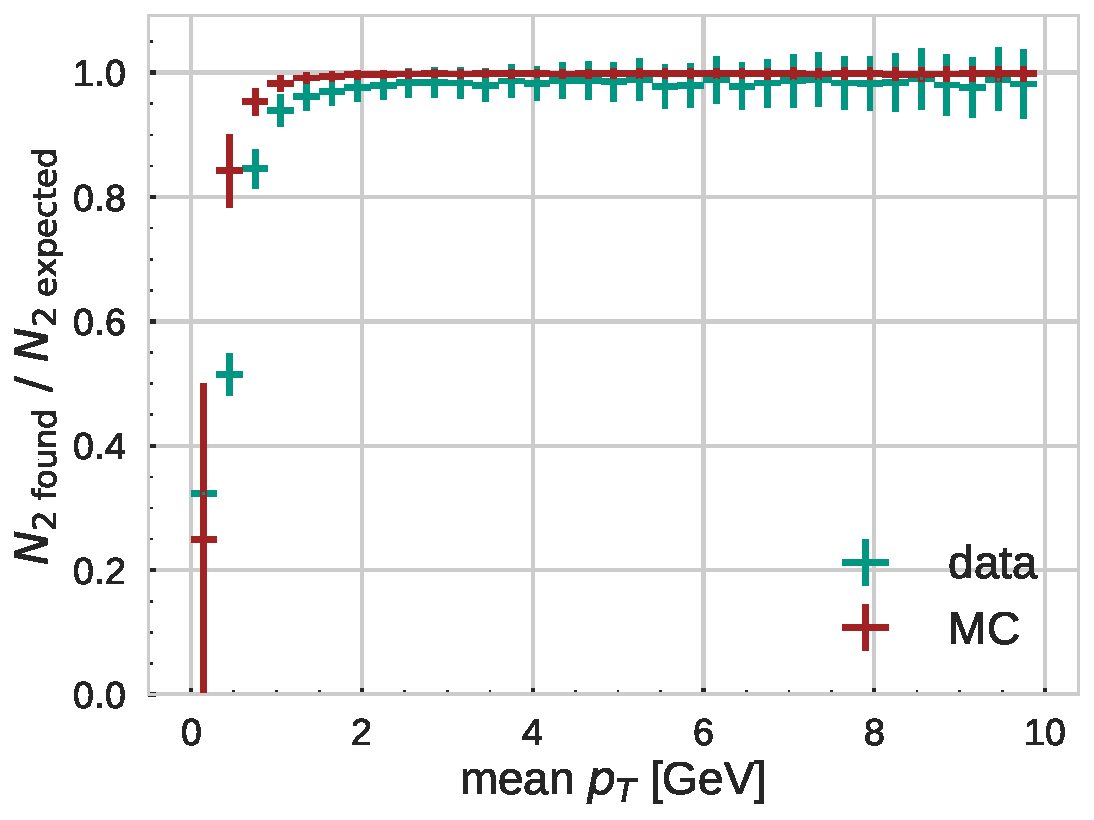
\includegraphics[width=0.85\textwidth]{figures/efficiency_study/cosmicbased_findeff_over_pt.pdf}
  \end{column}
  \begin{column}{0.5\textwidth}
    % \begin{itemize}
    % \item $>$ 1\,GeV very few finding fails
    % \item MC slightly better than data, especially at low $p_T$
    % \end{itemize}
  \end{column}
\end{columns}
\end{frame}

\begin{frame}
  \frametitle{Effizienz-Profil in weiteren Spurparametern}
  \begin{columns}
    \begin{column}{0.5\textwidth}
      \centering
      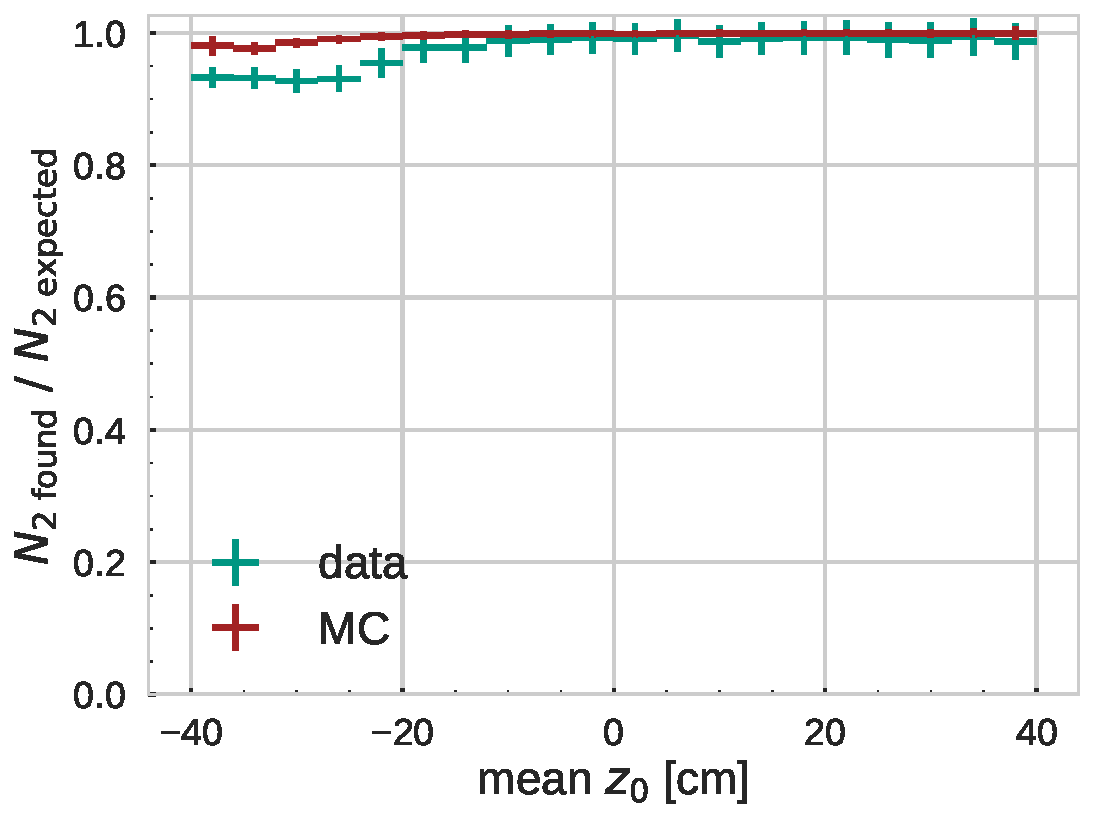
\includegraphics[width=0.85\textwidth]{figures/efficiency_study/cosmicbased_findeff_over_z0.pdf}\\
      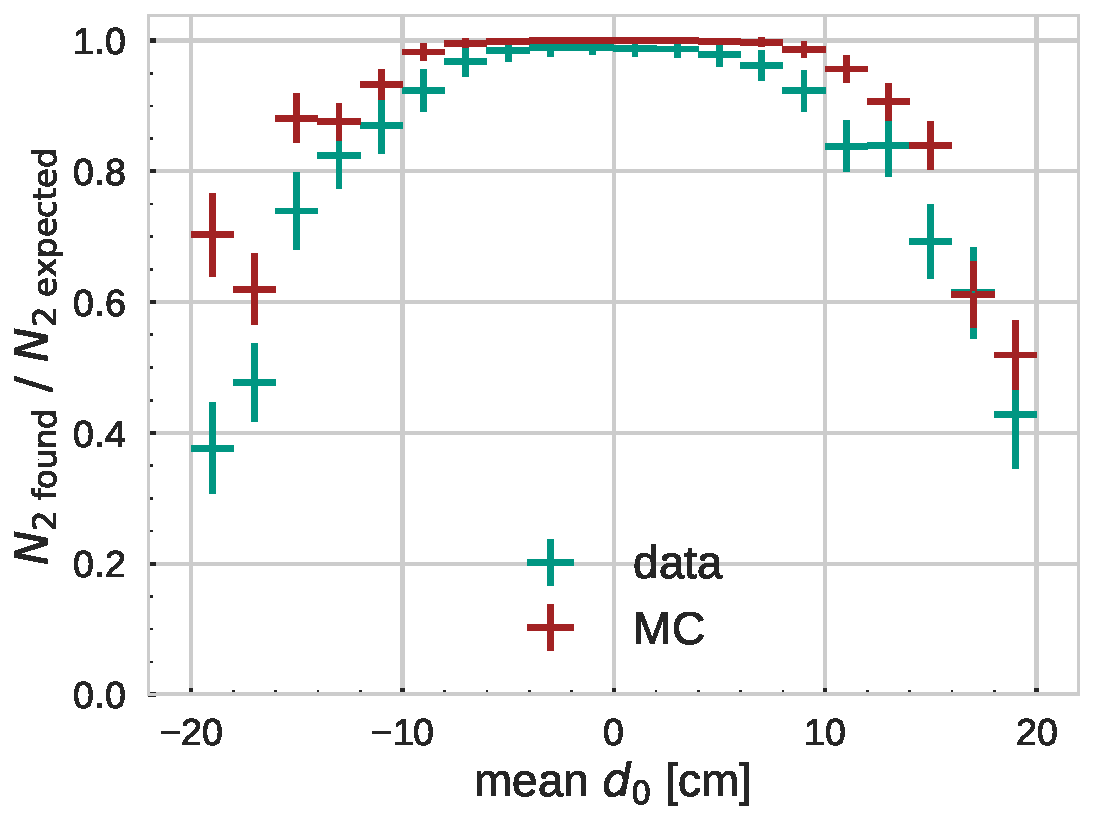
\includegraphics[width=0.85\textwidth]{figures/efficiency_study/cosmicbased_findeff_over_d0.pdf}
      
    \end{column}
    \begin{column}{0.5\textwidth}
      \centering
      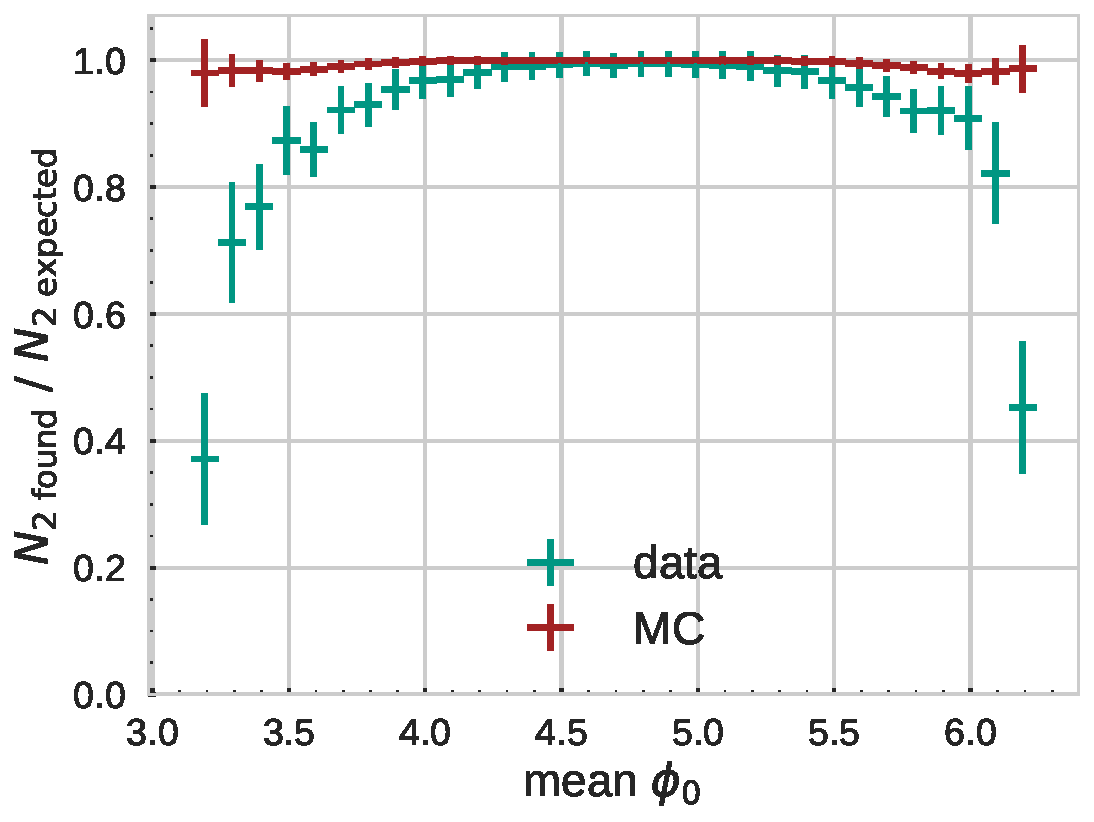
\includegraphics[width=0.85\textwidth]{figures/efficiency_study/cosmicbased_findeff_over_phi0.pdf}\\
      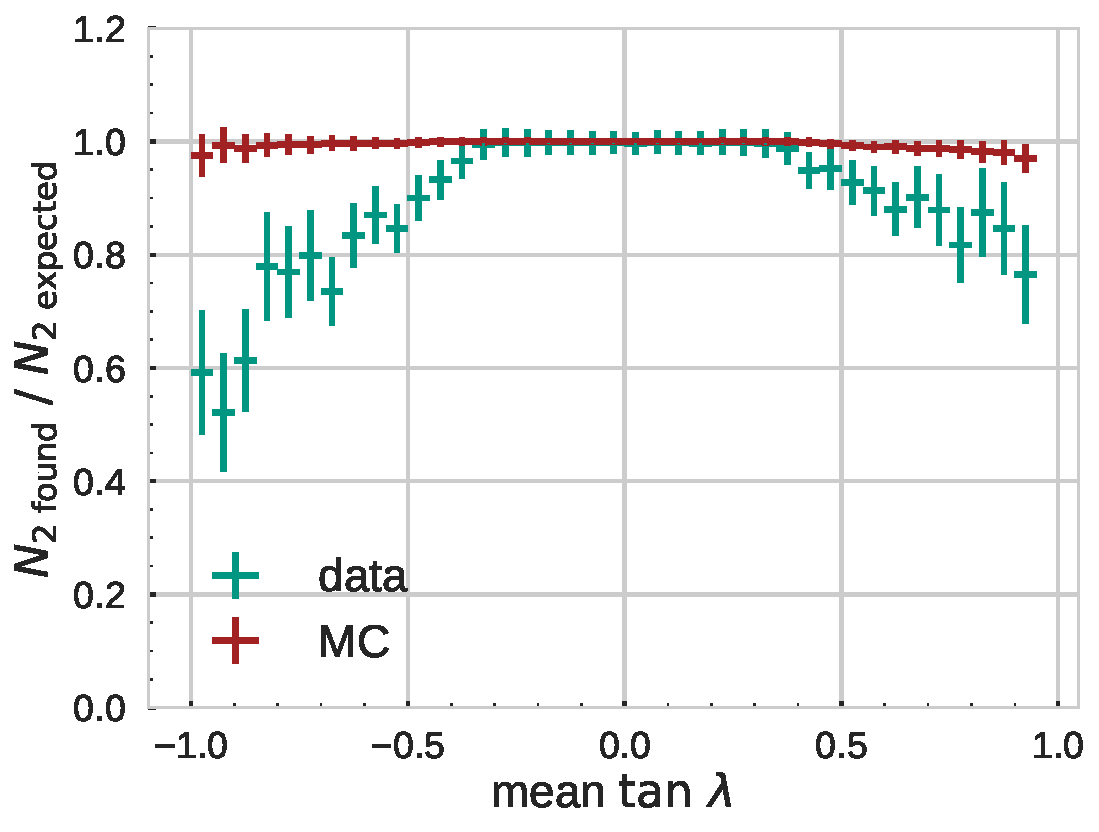
\includegraphics[width=0.85\textwidth]{figures/efficiency_study/cosmicbased_findeff_over_tan_lambda.pdf}
    \end{column}
  \end{columns}
\end{frame}

\begin{frame}
  \frametitle{Diskussion der Resultate}
  \begin{itemize}
  \item GOOD: Generally, finding fails very rare\\
    $\rightarrow$  \textbf{Confirmation that tracking works on on real data!}
  \item Many events where only one track is found are in low $p_T$ regions and extreme track parameter regions.
    In these regions are large differences between MC and data
  \item Cuts based on $\sum y$ assume almost straight track coming from above. We have seen that this does not always work, which might explain this low ``efficiencies'' in these regions.
  \item Seen in event displays and track parameter differences between both track halves:
    Often bad hit efficiencies and bad fit results. Only due to use of only half lengths (Glückstern Formula)?
  \end{itemize}
  
\end{frame}

\begin{frame}
  \frametitle{Ausblick}\label{lastbeforebackup}
  \begin{itemize}
  \item Increase trust on selection of events where we expect two tracks
    \\$\rightarrow$ further cuts?
  \item Compare with finding efficiency from MC matching? Difficult, because it works only well for merged tracks.
  \item Use new GCR MC sample with large 8\,m acceptox. Do differences between MC and data remain?
  \item Use cosmics to estimate hit efficiency. Create efficiency map?
  \end{itemize}
\end{frame}

  



\end{document}

%%% Local Variables:
%%% mode: latex
%%% TeX-master: t
%%% End:
